\section{Introducción}

En muchos problemas de optimización combinatoria es necesario encontrar la forma más eficiente de conectar un conjunto de nodos dentro de una red. 
Una herramienta fundamental para resolver este tipo de problemas es el \textit{Árbol Generador de Costo Mínimo} (Minimum Cost Spanning Tree, MST). 
Este consiste en un subconjunto de aristas de un grafo conexo que conecta todos los vértices sin formar ciclos y cuyo costo total es mínimo. 
El estudio de los MST es importante en diversas aplicaciones como el diseño de redes de comunicación, redes eléctricas y sistemas de transporte. 
Para resolver este problema existen algoritmos eficientes basados en estrategias voraces, entre los más conocidos se encuentran los algoritmos de Kruskal, Prim y Sollin, los cuales construyen el árbol seleccionando progresivamente las aristas de menor costo sin generar ciclos en la estructura. 
Estos métodos permiten encontrar soluciones óptimas de manera eficiente incluso para grafos de gran tamaño. 

\begin{itemize}

\item \textbf{Algoritmo de Kruskal:} 
Ordena todas las aristas del grafo de menor a mayor costo y las va agregando al árbol siempre que no formen un ciclo. 
El proceso continúa hasta que se han seleccionado $n-1$ aristas, formando así el árbol.

\item \textbf{Algoritmo de Prim:} 
Comienza con un vértice cualquiera y va construyendo el árbol agregando en cada paso la arista de menor costo que conecta un vértice del árbol con un vértice que aún no pertenece a él.

\item \textbf{Algoritmo de Sollin:} 
Inicia con un bosque donde cada vértice es un componente independiente. 
En cada iteración, cada componente selecciona la arista de menor costo que lo conecta con otro componente, fusionando los componentes hasta formar un único árbol.

\end{itemize}

En esta ocacion, se abordará el problema de encontrar el árbol generador de costo mínimo para un grafo dado, utilizando los 3 algoritmos mencionados 
y comparando sus resultados.

\begin{figure}[H]
    \centering
    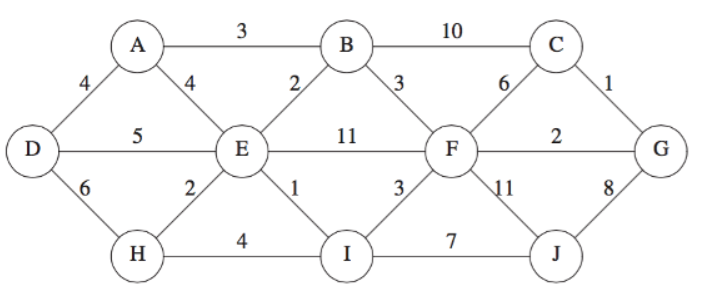
\includegraphics[width=0.75\textwidth]{rsc/img/base_tree.png}
    \caption{Grafo a resolver}\label{fig:base_Tree}
\end{figure}